%% start of file `template.tex'.
%% Copyright 2006-2015 Xavier Danaux (xdanaux@gmail.com), 2020-2021 moderncv maintainers (github.com/moderncv).
%
% This work may be distributed and/or modified under the
% conditions of the LaTeX Project Public License version 1.3c,
% available at http://www.latex-project.org/lppl/.


\documentclass[11pt,a4paper,sans]{moderncv}        % possible options include font size ('10pt', '11pt' and '12pt'), paper size ('a4paper', 'letterpaper', 'a5paper', 'legalpaper', 'executivepaper' and 'landscape') and font family ('sans' and 'roman')

% moderncv themes
\moderncvstyle{classic}                             % style options are 'casual' (default), 'classic', 'banking', 'oldstyle' and 'fancy'
\moderncvcolor{blue}                               % color options 'black', 'blue' (default), 'burgundy', 'green', 'grey', 'orange', 'purple' and 'red'
%\renewcommand{\familydefault}{\sfdefault}         % to set the default font; use '\sfdefault' for the default sans serif font, '\rmdefault' for the default roman one, or any tex font name
%\nopagenumbers{}                                  % uncomment to suppress automatic page numbering for CVs longer than one page

% character encoding
%\usepackage[utf8]{inputenc}                       % if you are not using xelatex ou lualatex, replace by the encoding you are using
%\usepackage{CJKutf8}                              % if you need to use CJK to typeset your resume in Chinese, Japanese or Korean

% adjust the page margins
\usepackage[scale=0.75]{geometry}
\usepackage{multicol}
\usepackage[
backend=biber,
style=numeric,
sorting=ydnt
]{biblatex}

\usepackage{fontspec}
\setmainfont{Montserrat Light}
 
\addbibresource{adonath-cv.bib}

%\usepackage{enumitem}

%\setlength{\hintscolumnwidth}{3cm}                % if you want to change the width of the column with the dates
%\setlength{\makecvheadnamewidth}{10cm}            % for the 'classic' style, if you want to force the width allocated to your name and avoid line breaks. be careful though, the length is normally calculated to avoid any overlap with your personal info; use this at your own typographical risks...


% personal data
\name{Axel}{Donath}
\title{Curriculum Vitae}                               % optional, remove / comment the line if not wanted
%\address{street and number}{postcode city}{country}% optional, remove / comment the line if not wanted; the "postcode city" and "country" arguments can be omitted or provided empty
%\phone[mobile]{+1~(234)~567~890}                   % optional, remove / comment the line if not wanted; the optional "type" of the phone can be "mobile" (default), "fixed" or "fax"
%\phone[fixed]{+2~(345)~678~901}
%\phone[fax]{+3~(456)~789~012}
\email{axeldonath@gmail.com}                               % optional, remove / comment the line if not wanted
%\homepage{www.johndoe.com}                         % optional, remove / comment the line if not wanted

% Social icons
\social[linkedin]{https://linkedin.com/in/axeldonath}                        % optional, remove / comment the line if not wanted
%\social[xing]{john\_doe}                           % optional, remove / comment the line if not wanted
%\social[twitter]{jdoe}                             % optional, remove / comment the line if not wanted
\social[github]{adonath}                              % optional, remove / comment the line if not wanted
%\social[gitlab]{jdoe}                              % optional, remove / comment the line if not wanted
%\social[stackoverflow]{0000000/johndoe}            % optional, remove / comment the line if not wanted
%\social[bitbucket]{jdoe}                           % optional, remove / comment the line if not wanted
%\social[skype]{jdoe}                               % optional, remove / comment the line if not wanted
\social[orcid]{0000-0003-4568-7005}                  % optional, remove / comment the line if not wanted
%\social[researchgate]{jdoe}                        % optional, remove / comment the line if not wanted
%\social[researcherid]{jdoe}                        % optional, remove / comment the line if not wanted
%\social[telegram]{jdoe}                            % optional, remove / comment the line if not wanted
%\social[googlescholar]{googlescholarid}                % optional, remove / comment the line if not wanted


%\extrainfo{additional information}                 % optional, remove / comment the line if not wanted
%\quote{Some quote}                                 % optional, remove / comment the line if not wanted

% bibliography adjustments (only useful if you make citations in your resume, or print a list of publications using BibTeX)
%   to show numerical labels in the bibliography (default is to show no labels)
%\makeatletter\renewcommand*{\bibliographyitemlabel}{\@biblabel{\arabic{enumiv}}}\makeatother
\renewcommand*{\bibliographyitemlabel}{[\arabic{enumiv}]}
%   to redefine the bibliography heading string ("Publications")
%\renewcommand{\refname}{Articles}

\usepackage{datetime}
\usepackage{amssymb}

\newdateformat{monthyeardate}{%
  \monthname[\THEMONTH], \THEYEAR}


\cfoot{\textcolor{gray}{Updated \monthyeardate\today}}

% bibliography with mutiple entries
%\usepackage{multibib}
%\newcites{book,misc}{{Books},{Others}}
%----------------------------------------------------------------------------------
%            content
%----------------------------------------------------------------------------------
\begin{document}
%\begin{CJK*}{UTF8}{gbsn}                          % to typeset your resume in Chinese using CJK
%-----       resume       ---------------------------------------------------------
\makecvtitle

\centering\textcolor{color1}{\rule{\textwidth}{1pt}}
\vspace*{-11pt}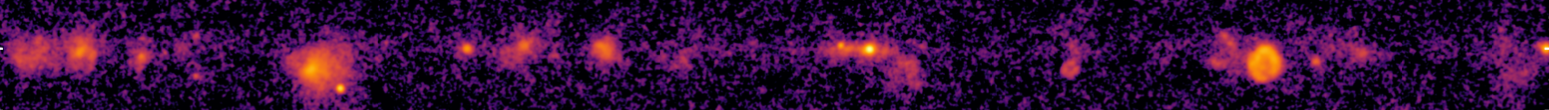
\includegraphics[width=\textwidth]{galactic-plane}
\centering\textcolor{color1}{\rule{\textwidth}{1pt}}

\begin{multicols}{2}
\begin{itemize}
\item[\small\textcolor{color1}{$\blacksquare$}] I am a Postdoc researcher at the Center for Astrophysics Harvard \& Smithsonian in Cambridge MA, where I research in the field of X-ray and gamma-ray astromomy.
\item[\small\textcolor{color1}{$\blacksquare$}] I am interested in the global structure of the Milky-Way in GeV-TeV gamma-rays and the Galactic gamma-ray source population. This includes association and classification of TeV gamma-ray sources in context of source catalog production as well as separation of sources from interstellar diffuse gamma-ray emission.   
\item[\small\textcolor{color1}{$\blacksquare$}] My second interest is in advanced data analysis methods for counts based data with low statistics. This includes maximum likelihood based spectro morphological modelling of gamma-ray data, with handling of time and spatially dependent instrument response and combining data from multiple gamma-ray instruments. 
\item[\small\textcolor{color1}{$\blacksquare$}] I am also interested in open source software development for astronomical data analysis and reproducible, open science.
\end{itemize}
\end{multicols}

\centering\textcolor{color1}{\rule{\textwidth}{1pt}}

\section{\textbf{Education}}
\cventry{\textbf{Phd} \\ \textcolor{gray}{2014 - 2018}}{Department of Physics and Astronomy}{Thesis: \textit{The Galactic Gamma-ray source Population between 10~GeV and 50~TeV}, advised by Werner Hofmann}{University of Heidelberg}{}{}  % Arguments not required can be left empty
\cventry{\textbf{M.Sc.} \\ \textcolor{gray}{2011 - 2014}}{Department of Physics and Astronomy}{Thesis: \textit{Towards the H.E.S.S. Galactic Plane Survey Catalog}, advised by Werner Hofmann}{University of Heidelberg}{}{}  % Arguments not required can be left empty
\cventry{\textbf{B.Sc.} \\ \textcolor{gray}{2007 - 2011}}{Department of Physics and Astronomy}{Specialized in Astronomy and Image Processing}{University of Heidelberg}{}{}

\section{\textbf{Experience}}

\subsection{Employment}
%------------------------------------------------
\cvitem{\textbf{CfA} \\ \textcolor{gray}{2021--present}}{Postdoctoral researcher, CHASC astro-statistic group, Center for Astrophysics Harvard \& Smithsonian, Cambridge MA. Supervised by Aneta Siemiginowska}
\cvitem{\textbf{MPIK} \\ \textcolor{gray}{2018--2021}}{Postdoctoral researcher, non-thermal astrophysics, Max-Planck-Institut for Nuclear Physics (MPIK), Heidelberg. Supervised by Jim Hinton}
\cvitem{\textbf{MPIK} \\ \textcolor{gray}{2014--2018}}{PhD student, high energy astrophysics, Max-Planck-Institut for Nuclear Physics (MPIK), Heidelberg. Supervised by Werner Hofmann}
\cvitem{\textbf{HCI} \\ \textcolor{gray}{2012--2014}}{Student assistent, computer vision, Heidelberg Collaboratory for Image Processing (HCI), Heidelberg. Supervised by Bernd Jähne.}
\cvitem{\textbf{Halle02} \\ \textcolor{gray}{2006--2007}}{Voluntary year in culture at \textit{Atelier Kontrast}, Heidelberg}
%------------------------------------------------

\subsection{Formal Teaching}
\cvitem{\textbf{Python} \\ \textcolor{gray}{Spring 2016}}{Tutor for \textit{Python programming for scientists}, lectured by Thomas Robitaille, University of Heidelberg}
\cvitem{\textbf{Python} \\ \textcolor{gray}{Fall 2015}}{Tutor for \textit{Python programming for scientists},
lectured by Thomas Robitaille, University of Heidelberg}
\cvitem{\textbf{Soft skills} \\ \textcolor{gray}{Autumn 2009}}{Tutor for \textit{Basiskurs Schl\"usselkompetenzen}, University of  Heidelberg}

\subsection{Service}
\cvitem{\textbf{PyGamma19} \\ \textcolor{gray}{2019}}{Member of the SoC and LoC for the 1st Python in Gamma-Ray Astronomy conference}
\cvitem{\textbf{PyGamma15} \\ \textcolor{gray}{2015}}{Member of the SoC and LoC for the 2nd Python in Gamma-Ray Astronomy conference}
\cvitem{\textbf{Gammapy} \\ \textcolor{gray}{2015-present}}{Organisation of mutiple Gammapy coding sprints (approx. 3 per year) and weekly Gammapy developer calls}
\cvitem{\textbf{JOSS} \\ \textcolor{gray}{August 2022-present}}{I am editor for the astronomy and astrophysics track of the Journal of Open Source Software}


\subsection{Mentoring}
\cvitem{\textbf{GSoC} \\ \textcolor{gray}{Summer 2015}}{Mentoring of Google Summer of Code project by Patti Carroll \textit{Astropy: Efficient and Precise Model Rasterization}.}


%----------------------------------------------------------------------------------------
%	AWARDS SECTION
%----------------------------------------------------------------------------------------

\section{\textbf{Awards}}
\cvitem{\textbf{ICVS} \\ \textcolor{gray}{June 2013}}{Recipient of the \textit{Best Paper Award} at the International Conference on Computer Vision Systems for the contribution \textit{Is Crowdsourcing feasible for optical flow ground truth estimation?}}

\cvitem{\textbf{ICRC} \\ \textcolor{gray}{July 2021}}{Recipient of the \textit{Best Poster Award} at the International Cosmic Ray Conference \textit{Gammapy: A Python Package for Gamma-Ray Astronomy}}.

\cvitem{\textbf{Open Science Award} \\ \textcolor{gray}{Dec 2021}}{Recipient of the Jury Price at the Open Science Awards for Open-Source Research Software from the French ministry of higher education with the Gammapy project}.


%----------------------------------------------------------------------------------------
%	COMPUTER SKILLS SECTION
%----------------------------------------------------------------------------------------

\section{\textbf{Computing}}
\cvitem{}{I am developer, maintainer and contributor to several astronomical Python software packages. See my GitHub profile \url{https://github.com/adonath} for an overview of my activity.}

\subsection{Skills}
\cvitem{Expert}{\textsc{Python},  \textsc{Numpy}, \textsc{Scipy}, \textsc{Matplotlib}, \textsc{Scikit-Learn}, \textsc{Scikit-Image}, \textsc{PyQt}, \textsc{Astropy}, \textsc{Pytorch}}
\cvitem{Intermediate}{\textsc{C++}, \LaTeX, \textsc{Linux}}
\cvitem{General}{\textsc{Git}, \textsc{Pytest}, \textsc{Sphinx}}

\subsection{Software}
\cvitem{\textbf{GSoC} \\ \textcolor{gray}{Summer 2013}}{Google Summer of Code project: \textit{AstroPy: Extending the functionality of the photutils package}, supervised by Thomas Robitaille}
\cvitem{\textbf{Gammapy} \\ \textcolor{gray}{2012-present}}{I am co-creator and currently lead developer of \href{https://gammapy.org}{Gammapy}, a Python package for Gamma-Ray astronomy and prototype for the science tools of the Cherenkov Telescope Array}
\cvitem{\textbf{Astropy} \\ \textcolor{gray}{2014-present}}{I have contributed multiple components to the convolution functionality of \href{https://www.astropy.org}{Astropy} a community developed Python package for astronomy. I am currently one of the sub-package maintainers of the Astropy convolution sub package.}
\cvitem{\textbf{gamma-cat} \\ \textcolor{gray}{2016-present}}{I am co-creator and maintainer of \href{https://github.com/gammapy/gamma-cat}{gamma-cat}, an open data collection and source catalog for gamma-ray astronomy.}


\cvitem{\textbf{Others} \\ \textcolor{gray}{2014-present}}{I have made mutiple minor contributions to Astropy affiliated packages \href{https://github.com/astropy/photutils}{photutils}, \href{https://github.com/astropy/regions}{regions} and \href{https://github.com/hipspy/hips}{hipspy}. I wrote the initial prototype for \href{https://scikit-image.org/docs/dev/auto_examples/features_detection/plot_blob.html}{Scikit-image's blob detection} functionality.}


\section{\textbf{Talks}}
\subsection{Astronomy}
\cvitem{\textbf{Gamma} \\ \textcolor{gray}{June 2016}}{\textit{The H.E.S.S. Galactic Plane Survey}, 6th International Symposium on High-Energy Gamma-Ray Astronomy, Heidelberg}
\cvitem{\textbf{TeVPa} \\ \textcolor{gray}{June 2016}}{\textit{The H.E.S.S. Galactic Plane Survey}, TeV Particle Astrophysics conference, Geneva}
\cvitem{\textbf{H.E.S.S.}\\ \textcolor{gray}{2014-2018}}{Various presentations on the H.E.S.S. Galactic Plane Survey at H.E.S.S. collaboration meetings, Warsaw, Heidelberg and Paris}


\subsection{Software}
\cvitem{}{\textcolor{gray}{* Invited talks / tutorials}}
\cvitem{\textbf{DAG} \\ \textcolor{gray}{Autumn 2014}}{\textit{Astropy - A community developed core package for Astronomy in Python}, German Astronomical Society (DAG), Bamberg}
\cvitem{\textbf{PyGamma15} \\ \textcolor{gray}{Nov. 2015}}{\textit{An overview of Astropy, Sherpa and Gammapy}, Python in Gamma Ray Astronomy Conference, Heidelberg}
\cvitem{\textbf{PyGamma19} \\ \textcolor{gray}{March 2019}}{\textit{Gammapy - A Python Package for Gamma-Ray Astronomy}, Python in Gamma Ray Astronomy Conference, Heidelberg}
\cvitem{\textbf{CTA/H.E.S.S.} \\ \textcolor{gray}{2014 -- 2019}}{Various Gammapy talks and tutorials at
H.E.S.S and CTA collaboration meetings, Annecy, Bologna and Lugano}
\cvitem{\textbf{*TU~Dortmund} \\ \textcolor{gray}{January 2021}}{\textit{Gammapy analysis methods and package}, Astroparticle Group Dortmund, Virtual}
\cvitem{\textbf{*HAWC} \\ \textcolor{gray}{June 2020}}{Gammapy analysis of public HAWC Crab data, HAWC technical meeting, Virtual}
\cvitem{\textbf{*Sexten} \\ \textcolor{gray}{June 2019}}{\textit{Gammapy} tutorial, Multimessenger Data Analysis in the CTA era Summer School, Sexten}
\cvitem{\textbf{*Asterics-Obelics} \\ \textcolor{gray}{2017--2019}}{Astropy tutorial, 1st, 2nd and 3rd ASTERICS-OBELICS International School, Annecy}


% \section{Skill matrix}
% \cvitem{Skill matrix}{Alternatively, provide a skill matrix to show off your skills}
% %% Skill matrix as an alternative to rate one's skills, computer or other.

% %% Adjusts width of skill matrix columns.
% %% Usage \setcvskillcolumns[<width>][<factor>][<exp_width>]
% %% <width>, <exp_width> should be lengths smaller than \textwidth, <factor> needs to be between 0 and 1.
% %% Examples:
% % \setcvskillcolumns[5em][][]%    adjust first column. Same as \setcvskillcolumns[5em]
% % \setcvskillcolumns[][0.45][]%   adjust third (skill) column. Same as \setcvskillcolumns[][0.45]
% % \setcvskillcolumns[][][\widthof{``Year''}]%     adjust fourth (years) column.
% % \setcvskillcolumns[][0.45][\widthof{``Year''}]%
% % \setcvskillcolumns[\widthof{``Languag''}][0.48][]
% % \setcvskillcolumns[\widthof{``Languag''}]%

% %% Adjusts width of legend columns. Usage \setcvskilllegendcolumns[<width>][<factor>]
% %% <factor> needs to be between 0 and 1. <width> should be a length smaller than \textwidth
% %% Examples:
% % \setcvskilllegendcolumns[][0.45]
% % \setcvskilllegendcolumns[\widthof{``Legend''}][0.45]
% % \setcvskilllegendcolumns[0ex][0.46]% this is usefull for the banking style

% %% Add a legend if you are using \cvskill{<1-5>} command or \cvskillentry
% %% Usage \cvskilllegend[*][<post_padding>][<first_level>][<second_level>][<third_level>][<fourth_level>][<fifth_level>]{<name>}
% % \cvskilllegend % insert default legend without lines
% %\cvskilllegend*[1em]{}% adjust post spacing
% % \cvskilllegend*{Legend}%  Alternatively add a description string
% %% adjust the legend entries for other languages, here German
% % \cvskilllegend[0.2em][Grundkenntnisse][Grundkenntnisse und eigene Erfahrung in Projekten][Umfangreiche Erfahrung in Projekten][Vertiefte Expertenkenntnisse][Experte\,/\,Spezialist]{Legende}

% % % Alternative legend style with the first three skill levels in one column
% % % Usage \cvskillplainlegend[*][<post_padding>][<first_level>][<second_level>][<third_level>][<fourth_level>][<fifth_level>]{<name>}
% % \setcvskilllegendcolumns[][0.6]%  works for classic, casual, banking
% % \setcvskilllegendcolumns[][0.55]%  works better for oldstyle and fancy
% % \cvskillplainlegend{}
% % \cvskillplainlegend[0.2em][Grundkenntnisse][Grundkenntnisse und eigene Erfahrung in Projekten][Umfangreiche Erfahrung in Projekten][Vertiefte Expertenkenntnisse][Experte/Guru]{Legende}

% %% Add a head of the skill matrix table with descriptions.
% %% Usage \cvskillhead[<post_padding>][<Level>][<Skill>][<Years>][<Comment>]%
% \cvskillhead[-0.1em]%   this inserts the standard legend in english and adjust padding
% %% Adjust head of the skill matrix for other languages
% % \cvskillhead[0.25em][Level][F\"ahigkeit][Jahre][Bemerkung]

% %% \cvskillentry[*][<post_padding>]{<skill_cathegory>}{<0-5>}{<skill_name>}{<years_of_experience>}{<comment>}%
% %% Example usages:
% \cvskillentry*{Language:}{3}{Python}{2}{I'm so experienced in Python and have realised a million projects. At least.}
% \cvskillentry{}{2}{Lilypond}{14}{So much sheet music! Man, I'm the best!}
% \cvskillentry{}{3}{\LaTeX}{14}{Clearly I rock at \LaTeX}
% \cvskillentry*{OS:}{3}{Linux}{2}{I only use Archlinux btw}% notice the use of the starred command and the optional
% \cvskillentry*[1em]{Methods}{4}{SCRUM}{8}{SCRUM master for 5 years}
% %% \cvskill{<0-5>} command
% %% \cvitem{\textbackslash{cvskill}:}{Skills can be visually expressed by the \textbackslash{cvskill} command, e.g. \cvskill{2}}

% Publications from a BibTeX file without multibib
%  for numerical labels: \renewcommand{\bibliographyitemlabel}{\@biblabel{\arabic{enumiv}}}% CONSIDER MERGING WITH PREAMBLE PART
%  to redefine the heading string ("Publications"): \renewcommand{\refname}{Articles}
\nocite{*}
%\bibliographystyle{plain}
%\bibliography{adonath-cv}                        % 'publications' is the name of a BibTeX file
\printbibliography[title={Publications and Proceedings}]
%\printbibliography[type=, title={Proceedings}, heading=subbibliography]


% Publications from a BibTeX file using the multibib package
%\section{Publications}
%\nocitebook{book1,book2}
%\bibliographystylebook{plain}
%\bibliographybook{publications}                   % 'publications' is the name of a BibTeX file
%\nocitemisc{misc1,misc2,misc3}
%\bibliographystylemisc{plain}
%\bibliographymisc{publications}                   % 'publications' is the name of a BibTeX file

%\clearpage\end{CJK*}                              % if you are typesetting your resume in Chinese using CJK; the \clearpage is required for fancyhdr to work correctly with CJK, though it kills the page numbering by making \lastpage undefined
\end{document}


%% end of file `template.tex'.

